\chapter{Otisky JA3, JA4 a~jejich použití}
\label{chp:JA34}
Tato kapitola se zabývá pasivními metodami pro~identifikaci šifrované komunikace a~jejich vývojem od~\textit{JA3} k~\textit{JA4+}. 
S narůstajícím trendem šifrování v~síťovém provozu bylo třeba vyvinout způsob klasifikace či identifikace šifrovaných dat kvůli správě a~analýze komunikace. V~roce 2015 byla představena, dnes již populární až možná zastaralou, pasivní metodu tvorby otisků TLS spojení označovanou jako \textit{JA3} otisky\footnote{Více na~\url{https://github.com/salesforce/ja3}}. Tvůrci \textit{John~B.~Althouse}, \textit{Jeff~Atkinson} a~\textit{Josh~Atkins} v~rámci společnosti \textit{Salesforce} ve~své metodě využívají atributy \textit{Hello} zpráv \textit{TLS} spojení. S~příchodem nové verze \textit{TLS v1.3}, která šifruje všechny zprávy protokolu \textit{Handshake} po~odeslání \textit{Server Hello} a~umožňuje využívat jako transportní protokol \textit{QUIC}, stejně jako další změny, které ztěžují efektivní identifikaci, již nebylo možné aplikovat \textit{JA3} otisky pro~tato spojení.

Pro pasivní metody identifikace zabezpečené komunikace se tak objevuje další výzva. V~roce 2023 přichází na~řadu sada metod \textit{JA4+}\footnote{Více na~\url{https://github.com/FoxIO-LLC/ja4}}, od~stejných tvůrců, v~zastoupení firmy \textit{FoxIO}. Příklady využití těchto otisků zahrnují skenování pro~odhalení hrozeb, detekci malwaru, prevenci únosu relace, automatizaci dodržování předpisů, sledování polohy, detekci \textit{DDoS} útoků, seskupování hrozeb, detekci reverzních shellů a~mnoho dalších~\cite{Althouse2023}.

V následující sekci~\ref{sec:JA3} je představen koncept \textit{JA3} otisků a~jejich využití. Na~ni navazuje sekce~\ref{sec:JA4+}, která seznamuje se sadou metod \textit{JA4+} pro~identifikaci různých vlastností šifrovaných spojení, jejichž součástí jsou také \textit{JA4} otisky. Porovnání \textit{JA3} a~\textit{JA4} otisků lze nalézt v~podsekci~\ref{sec:compJA34}.

\section{JA3 otisky}
\label{sec:JA3}
JA3 (pojmenování vzniklo podle jmen tří hlavních tvůrců: \textbf{J}ohn B. \textbf{A}lthouse, \textbf{J}eff \textbf{A}tkinson a~\textbf{J}osh \textbf{A}tkins) je metoda tvorby otisku \textit{TLS} spojení, která se zaměřuje na~různé aspekty a~atributy \textit{TLS handshake}. Používá hodnoty ze zpráv \textit{Client Hello} či \textit{Server Hello}, které obsahují několik detailů, jež dokážou jedinečně charakterizovat jak klienta, tak server. Po~extrakci těchto informací jsou jednotlivé hodnoty zřetězeny a~je proveden výpočet haše typu \textit{MD5}. Výstup hashovací funkce představuje zmíněný \textit{JA3} otisk, který poskytuje konzistentní a~identifikovatelný podpis.


Metoda \textit{JA3} využívá následující atributy \textit{Client Hello}: \texttt{client\_version}, \texttt{cipher\_suite}, \texttt{extensions}, \texttt{supported\_groups}\footnote{Dříve definováno jako \texttt{elliptic\_curves}} a~\texttt{ec\_point\_formats}\footnote{Dříve definováno jako \texttt{elliptic\_curve\_point\_formats}}. Pro~podrobnější popis těchto polí zprávy viz.~sekce~\ref{sec:clienthello}. Tyto hodnoty jsou pak spojeny dohromady v~uvedeném pořadí, přičemž jednotlivá pole jsou oddělena čárkou (`,`) a~hodnoty v~rámci každého pole jsou odděleny pomlčkou (`--`). Musí být brány v~potaz také hodnoty \textit{GREASE}; bližší popis lze nalézt v~sekci~\ref{sec:tls-13}. Při~extrakci hodnot z~polí jsou buďto ignorovány, nebo nahrazeny konstantou, aby byla zachována konzistence otisku.

Pro lepší porozumění je předvedena názorná ukázka, převzata z~\cite{Althouse2022JA3}.
Řetězec po~zpracování všech výše zmíněných polí vypadá následovně. Tento řetězec je poté použit jako vstup do~hashovací funkce \textit{MD5}, která vytvoří daný otisk.
\begin{table}[H]
	\centering
	\begin{tabular}{c|c}
		Řetězec & \verb|769,47–53–5–10–49161–49162–49171–49172–50–56–19–4,0–10–11,23–24,0| \\
		          & $\downarrow$                                                                                         \\
		Otisk     & \verb|ada70206e40642a3e4461f35503241d5|                                                              \\ 
	\end{tabular}
\end{table}

V případě, že nejsou žádná rozšíření dostupná, pole jsou ponechána prázdná:
\begin{table}[H]
	\centering
	\begin{tabular}{c|c}
		Řetězec & \verb|769,4–5–10–9–100–98–3–6–19–18–99,,,| \\        
		          & $\downarrow$                                                   \\
		Otisk     & \verb|de350869b8c85de67a350c8d186f11e6|                        \\ 
	\end{tabular}
\end{table}

Tato metoda se dá také aplikovat na~zprávu \textit{Server Hello} pro~identifikaci serveru. Jedná se o~takzvaný \textit{JA3S} otisk. Využívá hodnoty polí \texttt{server\_version}, \texttt{cipher\_suite} a~\texttt{extensions}, jak je podrobněji popsáno v~sekci~\ref{sec:serverhello}. Postup je poté totožný s~tvorbou otisku pro~klienta, a~to tedy zřetězením a~použitím jako vstupu pro~hashovací funkci \textit{MD5}.

Ukázka tvorby \textit{JA3S} otisku, také převzata z~\cite{Althouse2022JA3}:
\begin{table}[H]
	\centering
	\begin{tabular}{c|c}
		Řetězec & \verb|769,47,65281–0–11–35–5–16| \\        
		          & $\downarrow$                               \\
		Otisk     & \verb|4835b19f14997673071435cb321f5445|    \\ 
	\end{tabular}
\end{table}

V průběhu času se však ukázalo, že \textit{JA3} otisky již nejsou tak přesné, jak bylo potřeba, a~to z~následujících důvodů:
\begin{itemize}
	\item \textbf{Náhodné uspořádání TLS rozšíření}: Některé prohlížeče začaly náhodně měnit pořadí rozšíření za~účelem zmaření snah o~identifikaci. \textit{JA3} otisky se spoléhají na~sekvenční pořadí, které se náhodným řazením mění, což mělo za~důsledek \textbf{nespolehlivost} při~identifikaci jedinečných klientů.
	\item \textbf{Nekonzistence databází}: Implementace tvorby se lišily pro~různé programy a~databáze, což vedlo \textbf{k různým výsledkům pro~stejnou identifikovanou entitu}. Tato nejednotnost bránila efektivnímu a~spolehlivému sdílení otisků.
	\item \textbf{Omezený rozsah}: \textit{JA3} se zaměřovaly pouze na~prvky v~rámci \textit{Hello} zpráv \textit{TLS} spojení. Tento omezený rozsah často postrádal kontext o~prostředí klienta. Navíc, s~rostoucí popularitou novějších transportních protokolů, jako například \textit{QUIC}, se ukázalo, že \textbf{identifikace je neúčinná}.
\end{itemize}

\subsection{Spolehlivost a~omezení JA3 otisků}
Mobilních aplikací pomocí \textit{TLS} otisků lze považovat za~praktickou metodu s~potenciálním využitím v~digitální forenzní analýze. Studie ukázaly, že samotné použití \textit{JA3} otisku není pro~přesnou identifikaci mobilních aplikací dostačující. Spolehlivějších výsledků je dosaženo kombinací \textit{JA3}, \textit{JA3S} a~\textit{SNI}, přičemž všechny tyto charakteristiky lze jednoduše získat z~\textit{TLS} handshake zpráv~\cite{MatousekMobileDevice2020}. Rovněž byla zkoumána volatilita \textit{TLS} otisků \,--\, experimenty ukázaly, že jejich variabilita není výrazná~\cite{MatousekJA3Reliability2020}.

\subsection{Shrnutí a~přechod na~JA4+}
\textit{JA3} otisky poskytují jednoduchou a~rychlou identifikaci \textit{TLS} spojení; ovšem s~příchodem nové verze \textit{TLS 1.3} se stávají zastaralými a~jejich přesnost klesá. Řešením je využít jiné metody klasifikace nebo použít nového nástupce těchto otisků. V~následující sekci~\ref{sec:JA4+} je probírána sada metod \textit{JA4+}, která slouží jako novější verze \textit{JA3} a~přináší s~sebou také další možnosti analýzy, a~to nejen \textit{TLS} spojení.

\section{Sada metod JA4+}
\label{sec:JA4+}
Kvůli již zmíněným důvodům, které vedly k~nepřesnosti identifikace, byl vyvinut nástupce \textit{JA3} otisků, a~to \textit{JA4}. Přesněji se jedná o~sadu metod \textit{JA4+}, které dokáží identifikovat i~jinou komunikaci než pouze \textit{TLS}. V~této sadě se nachází jak metody \textit{JA4} a~\textit{JA4S} pro~tvorbu otisků \textit{TLS}, tak například \textit{JA4HTTP}, \textit{JA4Latency}, \textit{JA4SSH}, \textit{JA4TCP} a~další\dots V~rámci této práce je pozornost zaměřena pouze na~metody \textbf{JA4} a~\textbf{JA4S}.

\subsection{Metoda JA4}
\textit{JA4} přistupuje k~identifikaci podobně jako metoda JA3. Využívá určité hodnoty z~polí \textit{Hello} zpráv, které buď zřetězí, nebo z~nich vypočítá hash pomocí hashovací funkce \textit{SHA256}. Formát otisku je rozdělen do~tří částí (a, b, c), oddělených podtržítkem (\_). Každou z~těchto částí lze označit, což zjednodušuje použití v~situacích, kdy je k~identifikaci potřeba pouze konkrétní část~\cite{Althouse2023}. 

\subsection{Formát otisku JA4}
Tato podsekce se zaměřuje na~formát otisku \textit{JA4}. Na~základě uvedených příkladů lze vidět, jak je otisk strukturován a~z~jakých částí se skládá. Příklady formátu otisku jsou převzaty z~\cite{Althouse2023}. Formát otisku \textit{JA4} je následující:
\[
	\text{JA4} = \text{JA4a} \_ \text{JA4b} \_ \text{JA4c}
\]

Kde:
\begin{itemize}
	\item \textbf{JA4a} představuje konkatenaci vybraných informací o~TLS spojení, jako je:
	      \begin{itemize}
	      	\item Protokol, označený jako \texttt{\uv{t}} (\textit{TCP}) nebo \texttt{\uv{q}} (\textit{QUIC}),
	      	\item Verze TLS: 1.2 = \texttt{\uv{12}}, 1.3 = \texttt{\uv{13}},
	      	\item SNI, \texttt{\uv{d}} pro~doménu nebo \texttt{\uv{i}} pro~\textit{IP} adresu,
	      	\item Počet šifrovacích sad,
	      	\item Počet rozšíření,
	      	\item První hodnota \textit{ALPN}.
	      \end{itemize}
	      	      
	\item \textbf{JA4b} je zkrácený hash (12B) (\textit{SHA-256}) nad~seřazeným seznamem šifrovacích sad.
	      	      
	\item \textbf{JA4c} je také zkrácený hash (12B) (\textit{SHA-256}) nad~seřazeným seznamem rozšíření a~algoritmů pro~podpisy (\textit{signature algorithms}) v~pořadí, ve~kterém se objevují.
	      	      
\end{itemize}
Konkrétní příklad může vypadat takto:
\[
	\text{JA4} = \texttt{t13d1516h2} \_ \texttt{acb858a92679} \_ \texttt{e5627efa2ab1}
\]
	      
	      
Podobně jako u~svého předchůdce \textit{JA3}, umožňuje sada \textit{JA4} identifikaci serverové strany \textit{TLS} komunikace prostřednictvím analýzy zprávy \textit{Server Hello}. Tato zpráva, odesílaná v~nezašifrované formě, reflektuje volbu serveru na~základě parametrů uvedených v~předchozí zprávě \textit{Client Hello}. Obsahuje mimo jiné jednu šifrovací sadu vybranou ze seznamu nabízeného klientem a~sadu rozšíření, které server zvolil pro~navázání spojení. Formát otisku \textbf{JA4S} je obdobný:

\[
	\begin{aligned}
		\text{JA4S} & = \text{JA4Sa} \_ \text{JA4Sb} \_ \text{JA4Sc} 
	\end{aligned}
\]

Kde:
\begin{itemize}
	\item \textbf{JA4Sa} obsahuje následující vybrané hodnoty:
	      \begin{itemize}
	      	\item Protokol, označený jako \texttt{\uv{t}} (\textit{TCP}) nebo \texttt{\uv{q}} (\textit{QUIC}),
	      	\item Verze TLS: 1.2 = \texttt{\uv{12}}, 1.3 = \texttt{\uv{13}},
	      	\item Počet rozšíření,
	      	\item První hodnota \textit{ALPN}.
	      \end{itemize}
	      	      
	\item \textbf{JA4Sb} představuje zvolenou šifrovací sadu (\textit{cipher suite}).
	      	      
	\item \textbf{JA4Sc} je zkrácený hash (\textit{SHA-256}) nad~seřazeným seznamem rozšíření.
\end{itemize}

Konkrétní příklad může vypadat takto:
\[
	\begin{aligned}
		\text{JA4S} & = \text{t1204000} \_ \text{c030} \_ \text{4e8089b08790} 
	\end{aligned}
\]

\subsection{Využití otisků JA4}
Použitelnost \textit{JA4} otisku je různorodá. Přesná identifikace jednotlivých aplikací je stále obtížná. Otisk však dokáže poskytnout množinu možných kandidátů, přičemž mohutnost této množiny může být poměrně vysoká. I~přesto tato informace napomáhá přesnější klasifikaci~\cite{BurgetovaJA42024}. \textit{JA4} lze také využít pro~identifikaci škodlivých aplikací (\textit{malwaru}) v~síťovém provozu. Ukazuje se, že za~použití dalších informací o~TLS spojení, jako je kombinace \textit{JA4}, \textit{JA4S} a~\textit{SNI}, se přesnost detekce zlepšuje~\cite{MatousekJA4Malware2024}.

\section{Srovnání otisků JA3 a~JA4}
\label{sec:compJA34}
Pro účely porovnání je níže uveden zkrácený výpis z~\textit{TLS} spojení se zvýrazněním prvků, které jsou využívány v~otiscích \textit{JA3} a~\textit{JA4}. (Položka \texttt{Extensions} reprezentuje ostatní rozšíření, která nejsou jmenovitě využita ani v~jedné z~verzí \textit{JA} otisků.)

\paragraph{Legenda}
\begin{itemize}
	\item \colorbox{ForestGreen!30}{JA3} – prvek použitý pouze v~otisku JA3
	\item \colorbox{DodgerBlue!30}{JA4} – prvek použitý pouze v~otisku JA4
	\item \colorbox{Plum!30}{JA3 + JA4} – prvek společný pro~oba otisky
\end{itemize}

\begin{TLSDisplay}
	Transport Protocol : \colorbox{DodgerBlue!30}{TCP}
	Handshake Type: Client Hello (1)
	Version: \colorbox{Plum!30}{TLS 1.2} (0x0303)
	Cipher Suites Length: \colorbox{DodgerBlue!30}{34}
	\colorbox{Plum!30}{Cipher Suites} \colorbox{DodgerBlue!30}{(17 suites)}
	Compression Methods Length: 1
	Compression Methods (1 method)
	Extensions Length: \colorbox{DodgerBlue!30}{560}
	Extension: \colorbox{DodgerBlue!30}{server_name name=tasks-pa.clients6.google.com}
	Extension: \colorbox{ForestGreen!30}{elliptic_curves} (len=2)
	Extension: \colorbox{ForestGreen!30}{ec_point_formats} (len=2)
	Extension: \colorbox{DodgerBlue!30}{application_layer_protocol_negotiation} (len=14)
	Extension: \colorbox{DodgerBlue!30}{signature_algorithms} (len=24)
	\dots
	\colorbox{Plum!30}{Extensions\dots}
\end{TLSDisplay}


Jak je patrné, otisky \textit{JA4} využívají širší spektrum informací, například transportní protokol nebo konkrétní rozšíření \textit{TLS}, což vede k~jejich vyšší unikátnosti a~spolehlivější identifikaci klientů~\cite{Althouse2023}.  Rozdíl je také v~tom, jak se s~těmito atributy nakládá. Starší verze \textit{JA3} odebere tzv.~\textit{GREASE} hodnoty, spojí je v~daném pořadí, přičemž používá znak \uv{,} k~oddělení jednotlivých polí a~znak \uv{-} k~oddělení hodnot v~každém poli. Tento řetězec je poté vstupem pro~hashovací funkci \textit{MD5}~\cite{Althouse2022JA3}. Jak lze spatřit v~diagramu~\ref{fig:JA3-creation}, jednotlivé kroky tohoto procesu jsou znázorněny sekvenčně.

\begin{figure}[H]
	\centering
	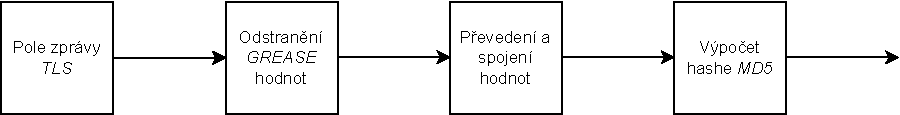
\includegraphics[width=\textwidth]{obrazky-figures/ja3-creation.drawio-crop.pdf}
	\caption{Proces tvorby otisků \textit{JA3}}
	\label{fig:JA3-creation}
\end{figure}
Novější verze \textit{JA4} vytváří otisky komplexnějším způsobem. První část otisku obsahuje zkonkatenizované hodnoty, druhá a~třetí část obsahují zkrácený hash \textit{SHA-256} nad~vybranými poli zprávy (seřazenými seznamy). Bližší popis je uveden v~sekci~\ref{sec:JA4+} nebo znázorněn diagramem~\ref{fig:JA4-creation}

\begin{figure}[H]
	\centering
	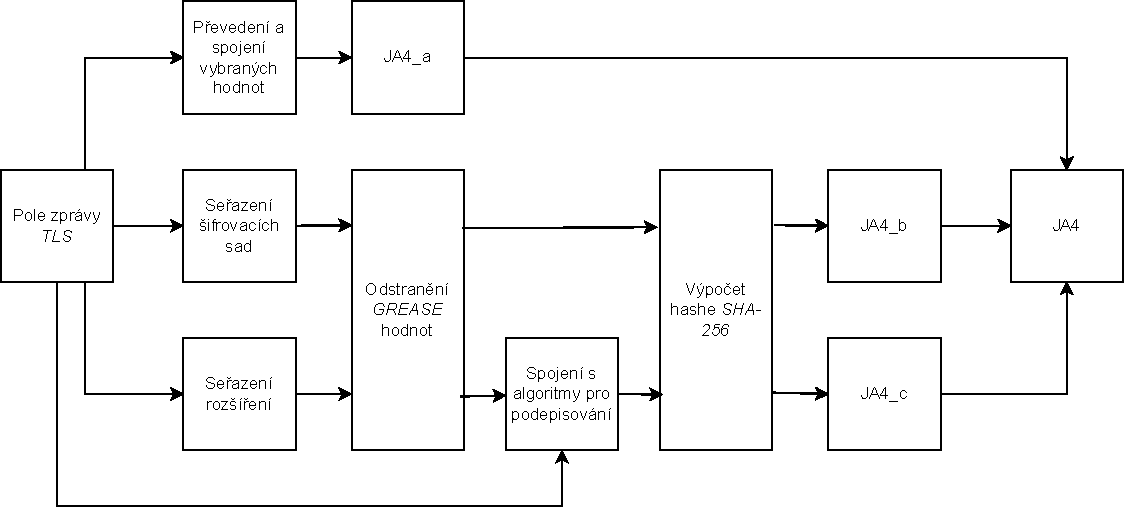
\includegraphics[width=\textwidth]{obrazky-figures/ja4-creation.drawio-crop.pdf}
	\caption{Proces tvorby otisků \textit{JA4}}
	\label{fig:JA4-creation}
\end{figure}

Z technického hlediska představuje sada metod \textit{JA4+} významný posun oproti svému předchůdci. Zatímco \textit{JA3} představuje jednoduchý a~stále využívaný nástroj, zaměřuje se pouze na~omezenou množinu atributů TLS zpráv. Naproti tomu \textit{JA4} zohledňuje širší spektrum informací, čímž zvyšuje unikátnost výsledného otisku.

Navíc \textit{JA4} implementuje vícefázový proces tvorby otisku – první část je tvořena explicitními hodnotami, následují hashované části, které zároveň eliminují vliv náhodného přehazování rozšíření a~šifrovacích sad. Použití \textit{SHA-256} namísto \textit{MD5} zvyšuje odolnost vůči kolizím.

Díky těmto změnám poskytuje \textit{JA4} výrazně přesnější identifikaci a~vyšší robustnost vůči technikám obfuskace, což z~něj činí užitečný nástroj pro~moderní síťovou analýzu.
